\documentclass[a4paper,12pt]{article} % добавить leqno в [] для нумерации слева
\usepackage[a4paper,top=1.3cm,bottom=2cm,left=1.5cm,right=1.5cm,marginparwidth=0.75cm]{geometry}
\def\picdir{./}
%%% Работа с русским языком
\usepackage{cmap}					% поиск в PDF
\usepackage[warn]{mathtext} 		% русские буквы в фомулах
\usepackage[T2A]{fontenc}			% кодировка
\usepackage[utf8]{inputenc}			% кодировка исходного текста
\usepackage[english,russian]{babel}	% локализация и переносы
\usepackage{physics}
\usepackage{multirow}
\usepackage{bm}
\usepackage{longtable}

%%% Нормальное размещение таблиц (писать [H] в окружении таблицы)
\usepackage{float}
\restylefloat{table}

\usepackage{graphicx}

\usepackage{wrapfig}
\usepackage{tabularx}

\usepackage{hyperref}
\usepackage[rgb]{xcolor}
\hypersetup{
  colorlinks=true,urlcolor=blue
}
\usepackage{pgfplots}
\pgfplotsset{compat=1.9}
%%% Дополнительная работа с математикой
\usepackage{amsmath,amsfonts,amssymb,amsthm,mathtools} % AMS
\usepackage{icomma} % "Умная" запятая: $0,2$ --- число, $0, 2$ --- перечисление

%% Номера формул
% \mathtoolsset{showonlyrefs=true} % Показывать номера только у тех формул, на которые есть \eqref{} в тексте,

%% Шрифты
\usepackage{euscript}	 % Шрифт Евклид
\usepackage{mathrsfs} % Красивый матшрифт

%% Свои команды
\DeclareMathOperator{\sgn}{\mathop{sgn}}

%% Перенос знаков в формулах (по Львовскому)
% \newcommand*{\hm}[1]{#1\nobreak\discretionary{}
%	{\hbox{$\mathsurround=0pt #1$}}{}}

\date{\today}

\usepackage{svg}
\newcommand{\svg}[3][0.7] {
  \begin{figure}[h]
    \begin{center}
      \fontsize{7}{8}\selectfont
      \includesvg[scale=#1]{\picdir #2}
      \caption{#3}
    \end{center}
  \end{figure}
}


\begin{document}

\begin{center}
  \footnotesize{ФЕДЕРАЛЬНОЕ ГОСУДАРСТВЕННОЕ АВТОНОМНОЕ ОБРАЗОВАТЕЛЬНОЕ 			УЧРЕЖДЕНИЕ ВЫСШЕГО ОБРАЗОВАНИЯ}\\
  \footnotesize{МОСКОВСКИЙ ФИЗИКО-ТЕХНИЧЕСКИЙ ИНСТИТУТ\\(НАЦИОНАЛЬНЫЙ 			ИССЛЕДОВАТЕЛЬСКИЙ УНИВЕРСИТЕТ)}\\
  \hfill \break
  \hfill \break
  \hfill \break
  \hfill \break
\end{center}


\begin{figure*}[h]
  \centering
  \includegraphics*[width=10cm,height=7cm,keepaspectratio]{mipt_eng_text_png.png}
  \label{fig:my_label}
\end{figure*}


\begin{center}   
  \hfill \break
  \hfill \break
  \hfill \break
  \large{Лабораторная работа № 3.4.5\\ \hfill \break\Large{Петля гистерезиса}}\\
  \hfill \break
  \hfill \break
  \hfill \break
  \hfill \break
  \begin{flushright}
    Юка Элож, Сирый Р.А.\\
    Б02-206
  \end{flushright}
  \hfill \break
  \hfill \break
  \hfill \break
\end{center}
\hfill \break
\hfill \break
\hfill \break
\hfill \break
\begin{center}
  Долгопрудный, 2023 г.
\end{center}
\thispagestyle{empty}

\newpage
\section{Введение}

\textbf{Цель работы:} изучение петель гистерезиса различных ферромагнитных
материалов в переменных полях.

\textbf{В работе используются:} автотрансформатор, понижающий трансформатор, интегрирующая цепочка, амперметр, вольтметр, электронный
осциллограф, делитель напряжения, тороидальные образцы с двумя обмотками.


\section{Теоретические сведения}

Основные характеристики
ферромагнетиков — их коэрцитивное поле $H_c$, магнитная проницаемость
$\mu$, рассеиваемая в виде тепла при перемагничивании мощность — зависят
от частоты перемагничивающего поля. В данной работе кривые гистерезиса ферромагнитных материалов изучаются в поле частоты $\nu_0 =$ 50 Гц
с помощью электронного осциллографа.
\begin{figure}[H]
  \centering
  \includegraphics{petlya.png}
  \caption{Петля гистерезиса ферромагнетика}
  \label{fig:petlya}
\end{figure}

Магнитная индукция $ B $ и напряжённость поля $ H $ в ферромагнитном материале неоднозначно связаны между собой: индукция зависит
не только от напряжённости, но и от предыстории образца. Связь между $ B $ и $ H $ типичного ферромагнетика иллюстрирует рис. $\ref{fig:petlya}$.

Если к ферромагнитному образцу прикладывать переменное внешнее
магнитное поле, то его состояние на плоскости $ B-H $ будет изменяться
по замкнутой кривой — петле гистерезиса. Размер петли определяется
максимальным значением напряжённости $ H $ в цикле (например, петля $ AA' $,
обозначенная пунктиром на рис. $\ref{fig:petlya}$). Если амплитуда напряжённости достаточно велика, то образец будет периодически достигать насыщения,
что на рисунке соответствует кривой $ CEFC'E'F'C $ (предельная петля
гистерезиса). Пересечение предельной петли с вертикальной осью соответствует остаточной индукции $B_r$, пересечение с горизонтальной осью
— коэрцитивному полю $H_c$. Крайние точки петель, соответствующие амплитудным значениям $ H $ (например, точка $ A $ на рис. $\ref{fig:petlya}$), лежат на начальной кривой намагничивания ($ OAC $).

\textbf{Измерение магнитной индукции.} Магнитную индукцию $ B $ удобно
определять с помощью ЭДС, возникающей при изменении магнитного
потока $ \Phi $ в катушке, намотанной на образец. Пусть катушка c $ N $ витками плотно охватывает образец сечением $ S $, и индукция $ B $ в образце
однородна. Тогда

\begin{equation}
  |B|=\frac{1}{SN}\int\mathcal{E} dt.
  \label{eq:|B|}
\end{equation}
\begin{wrapfigure}{r}{0.35\linewidth}
  \includegraphics[width=\linewidth]{int.png}
  \caption{Интегрирующая ячейка}
  \label{fig:int}
\end{wrapfigure}

Для интегрирования в работе используется интегрирующая $ RC $-цепочка (рис. $ \ref{fig:int} $).
«Входное» напряжение от источника $U_{\text{вх}}(t)$ подаётся на последовательно соединённые резистор $R_\text{и}$ и конденсатор $C_\text{и}$. <<Выходное>>
напряжение $U_{\text{вых}}(t)$ снимается с конденсатора. Предположим, что 1) сопротивление источника мало по сравнению с $R_\text{и}$, 2) выходное сопротивление (сопротивление на входе осциллографа), напротив, велико: $R_{\text{вых}}$ $ \gg $ $R_\text{и}$ и, наконец, 3) сопротивление $R_\text{и}$ достаточно велико, так что почти всё падение напряжения приходится на него, а $U_{\text{вых}}$ $\ll$ $U_{\text{вх}}$. В таком случае ток цепи равен I = ($U_{\text{вх}}$ - $U_{\text{вых}}$)/$R_\text{и}$ $\approx$ $U_{\text{вх}}$/$R_\text{и}$, и входное и выходное сопротивление связаны соотношением
\begin{equation}
  U_{\text{вых}} = \frac{q}{C_\text{и}} = \frac{1}{C_\text{и}}\int\limits_0^t Idt \approx \frac{1}{\tau_\text{и}} \int\limits_0^t U_{\text{вх}}dt,
  \label{eq:U_ext}
\end{equation}
где $\tau_\text{и}=R_\text{и}C_\text{и}$ - постоянная времени $ RC $ - цепочки. Для индукции поля из ($\ref{eq:|B|}$) получаем 
\begin{equation}
  |B|=\frac{1}{SN}\int U_{\text{вх}} dt=\frac{\tau_\text{и}}{SN}U_{\text{вых}}.
  \label{eq:|B|new}
\end{equation}

\textbf{Замечание.} Уточним критерий применимости соотношения ($\ref{eq:U_ext}$). Пусть на вход интегрирующей ячейки подан синусоидальный сигнал с частотой $\omega_0$. Тогда, пользуясь методом комплексных амплитуд, нетрудно найти отношение амплитуд входного и выходного напряжений:
\begin{equation}
  \frac{U_{\text{вых}}}{U_{\text{вх}}}=\frac{1/\omega_0C}{\sqrt{R^2+1/(\omega_0C)^2}}.
\end{equation}
Тогда неравенство $U_{\text{вых}} \ll U_{\text{вх}}$ реализуется, если 
\begin{equation}
  \tau \equiv RC\gg \frac{1}{\omega_0}
\end{equation}
(импеданс конденсатора мал по сравнению сопротивлением резистора).
В таком случае для синусоидального сигнала имеем
\begin{equation}
  \frac{U_{\text{вых}}}{U_{\text{вх}}}\approx\frac{1}{\omega_0\tau}.
\end{equation}
В общем случае, если $\omega_0$ — частота самой низкой гармоники в спектре
произвольного входного сигнала, то при $\omega_0\tau \gg 1$ неравенство $U_{\text{вых}} \ll U_{\text{вх}}$ выполняется на любой частоте $\omega > \omega_0$.

\section{Экспериментальная установка}

Схема установки изображена на рис. 3. Напряжение сети (220 В,
50 Гц) с помощью трансформаторного блока Т, состоящего из регулировочного автотрансформатора и разделительного понижающего трансформатора, подаётся на намагничивающую обмотку $N_0$ исследуемого образца.
\begin{figure}[h!]
  \centering
  \includegraphics{scheme.png}
  \caption{ Схема установки для исследования намагничивания образцов}
  \label{fig:scheme}
\end{figure}

В цепь намагничивающей катушки, на которую подаётся некоторое напряжение $U_0$,
последовательно включено сопротивление $R_0$. Напряжение на $R_0$, равное $U_R$=
$R_0I_0$, где $I_0$ — ток в намагничивающей обмотке $N_0$, подаётся на канал $ X
$ осциллографа. Связь напряжённости $ H $ в образце и тока $I_0$ рассчитывается
по теореме о циркуляции.  Действующее значение переменного тока в обмотке $N_0$
измеряется амперметром A.  Для измерения магнитной индукции $ B $ с
измерительной обмотки $N_\text{и}$ на вход $ RC $-цепочки подаётся напряжение
$U_\text{и}$ ($U_{\text{вх}}$), пропорциональное производной $ dB/dt $. С
интегрирующей ёмкости $C_\text{и}$ снимается напряжение $U_C$
($U_{\text{вых}}$), пропорциональное величине $ B $, и подаётся на вход $ Y $
осциллографа. Значение индукции поля $ B $ рассчитывается по формуле 3.
Замкнутая кривая, возникающая на экране, воспроизводит в некотором масштабе
(различном для осей $ X $ и $ Y $) петлю гистерезиса. Чтобы придать этой кривой
количественный смысл, необходимо установить масштабы изображения, т. е. провести
калибровку каналов $X$ и $Y$ осциллографа.

\section{Ход работы}
\subsection{Измерение петель гистерезиса}

\begin{enumerate}


\item Соберем схему согласно рис.3. Подберем ток питания в намагничивающей обмотке с помощью автотрансформатора и коэффициенты усиления ЭО таким образом, чтобы предельная петля гистерезиса занимала большую часть экрана. Приведем характерные значения катушек разных материалов в таблице 1.

  \begin{table}[H]
    \centering
    \begin{tabular}{|c|c|c|c|c|}
      \hline
      Материал     & $N_0$ & $N_\text{и}$ & $S^2$, см$^2$ & $2\pi R$, см \\ \hline
      Феррит       & 42    & 400                              & 3,00           & 25,0         \\ \hline
      Пермаллой    & 20    & 300                             & 0,76          & 13,3         \\ \hline
      Крем. железо & 25    & 250                             & 2,00          & 11,0         \\ \hline
    \end{tabular}
    \caption{Характеристики катушек}
    \label{tab:har_kat}
  \end{table}

\item Для каждого образца получим передельные петли гистерезиса, по коэффициентам усиления ЭО $K_x$ и $K_y$ рассчитаем масштабы, определим двойные амплитуды коэрцетивого поля $ [2x(c)] $, индукции насыщения $ [2y(r)]$, напряжённости $H_{s}$ ($ [2x(s)] $) и индукции $B_{s}$ ($ [2x(c)] $) . Результаты измерений и вычислений занесём в таблицу:

  \begin{table}
    \centering
    \begin{tabular}{|c|c|c|c|c|c|c|}
      \hline
      Материал     & $[2x(c)]$, дел & $[2y(r)]$, дел & $K_x$, мВ/дел & $K_y$, мВ/дел & $[2x(s)]$, дел  & $[2y(s)]$, дел \\ \hline
      Феррит       & 7,9            & 4,0            & 5            & 5    & 8,0 & 4,9 \\ \hline
      Пермаллой    & 5,2           & 6,4            & 5            & 5     &  9,6  & 6,6     \\ \hline
      Крем. железо & 7,8            & 5,7           & 5           & 5     & 10,0 & 6,5   \\ \hline
    \end{tabular}
  \end{table}

\item Найдём значения остаточной индукции $B_{r}$,индукции  и напряжённости коэрцитового поля $H_{r}$, а также $B_{s}$ и $H_{s}$ насыщения:

  \begin{table}[H]
    \centering
    \begin{tabular}{|c|c|c|c|c|c|c|}
      \hline
      Материал     & $I$, мА & $U_{вых}$, мВ & $H_{c}$, А$\cdot$м$^{-1}$ & $B_{r}$, Тл & $H_{r}$, А$\cdot$м$^{-1}$ &  $B_{s}$, Тл \\ \hline
      Феррит       & 640   &   602         & $107\pm2$ & 0,07   & п &   \\ \hline
      Пермаллой    & 77    &   603          & $12\pm1$ & 0,88   &  п &  \\ \hline
      Крем. железо & 169   &   607         & $38\pm4$   & 0,40   &  п &  \\ \hline
    \end{tabular}
    \caption{Результаты измерений}
    \label{tab:izm}
  \end{table}

  При определении индукции магнитного поля по формуле (3) были взяты значения $R_{и} = 200 \text{кОм}$ и $C_{и} = 20 \text{мкФ}$.

\item Плавно уменьшая амплитуду тока намагничивания до нуля, зафиксируем на осциллографи положения крайних точек наблюдаемых петель:


  \begin{figure}[h!]
    \centering
    \includegraphics[width=8cm]{11.jpeg}
    \caption{Предельная петля пермаллоя}
  \end{figure}
  \begin{figure}[h!]
    \centering
    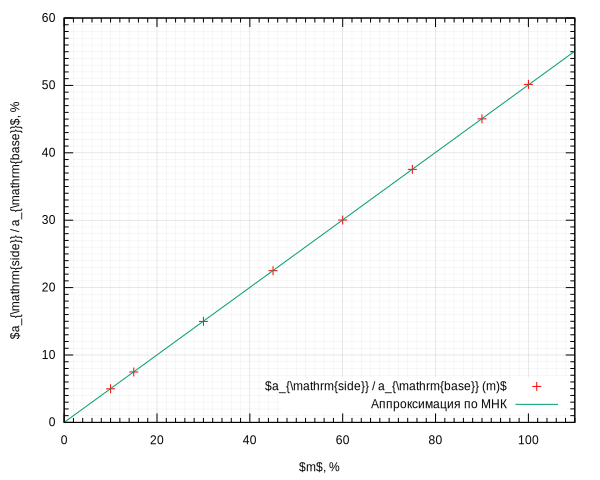
\includegraphics[width=8cm]{22.jpg}
    \caption{Предельная петля гистерезиса кремнитого железа}
  \end{figure}
  \newpage
  \begin{figure}[h!]
    \centering
    \includegraphics[width=8cm]{3333.jpg}
    \caption{Предельная петля гистерезиса феррита}
  \end{figure}

  По виду начальных кривых намагничивания получим начальные и конечные значения дифференциальной магнитной проницаемости $\mu_{диф}$:



  \begin{table}[H]
    \centering
    \begin{tabular}{|c|c|c|c|c|c|c|}
      \hline
      Вещество  &	$\mu_{диф}$ нач  & $\mu_{диф}$ макс  \\ \hline
      Феррит       & отгш          & 4уклдпьукьп        \\ \hline
      Пермаллой    & укпукщп         & кплкщп         \\ \hline
      Крем. железо & льукпь           & улкпк        \\ \hline
    \end{tabular}
  \end{table}




  \subsection{Проверка применимости теоретических выкладок}

  Проверим применимость формулы 2, разобрав цепь тороида, подав на ячейки синусоидальное напряжение и вычислив отношение входного и выходного напряжений: 

  \begin{equation}
    \tau_{и} = R_{и}C_{и} = 4 \text{ с}; \quad U_{вых}/U_{вх} \approx \frac{1}{2\pi\nu_{0}\tau} \approx 8\cdot 10^{-3} \ll 1
  \end{equation}

  Реальные показания дают $U_{вых}/U_{вх}\approx 0,8$ Данный результат означает, что...

  \subsection{Вывод, обсуждение результатов}

  Полученные значения ..... Продолжение следует...

\end{enumerate}

\svg{fesi.svg}{Say gex}

\end{document}
